\documentclass{beamer}

\usetheme{metropolis}

\metroset{
  progressbar=frametitle,   % thin progress bar under each title
  block=fill,
  numbering=fraction        % "3/12" instead of just "3"
}
\usepackage{graphicx}
\usepackage{booktabs}

\title{Case Studies: Sports Analytics}
\subtitle{UEFA Euro -- ML competition}
\author{Nicholas, Sriram, Rohit, Silas}
\date{}

\begin{document}

\maketitle


% ------------------------------------------------------------------
\begin{frame}
  \frametitle{Nested CV}
  
    \begin{columns}[c]
        \begin{column}{0.5\textwidth}
            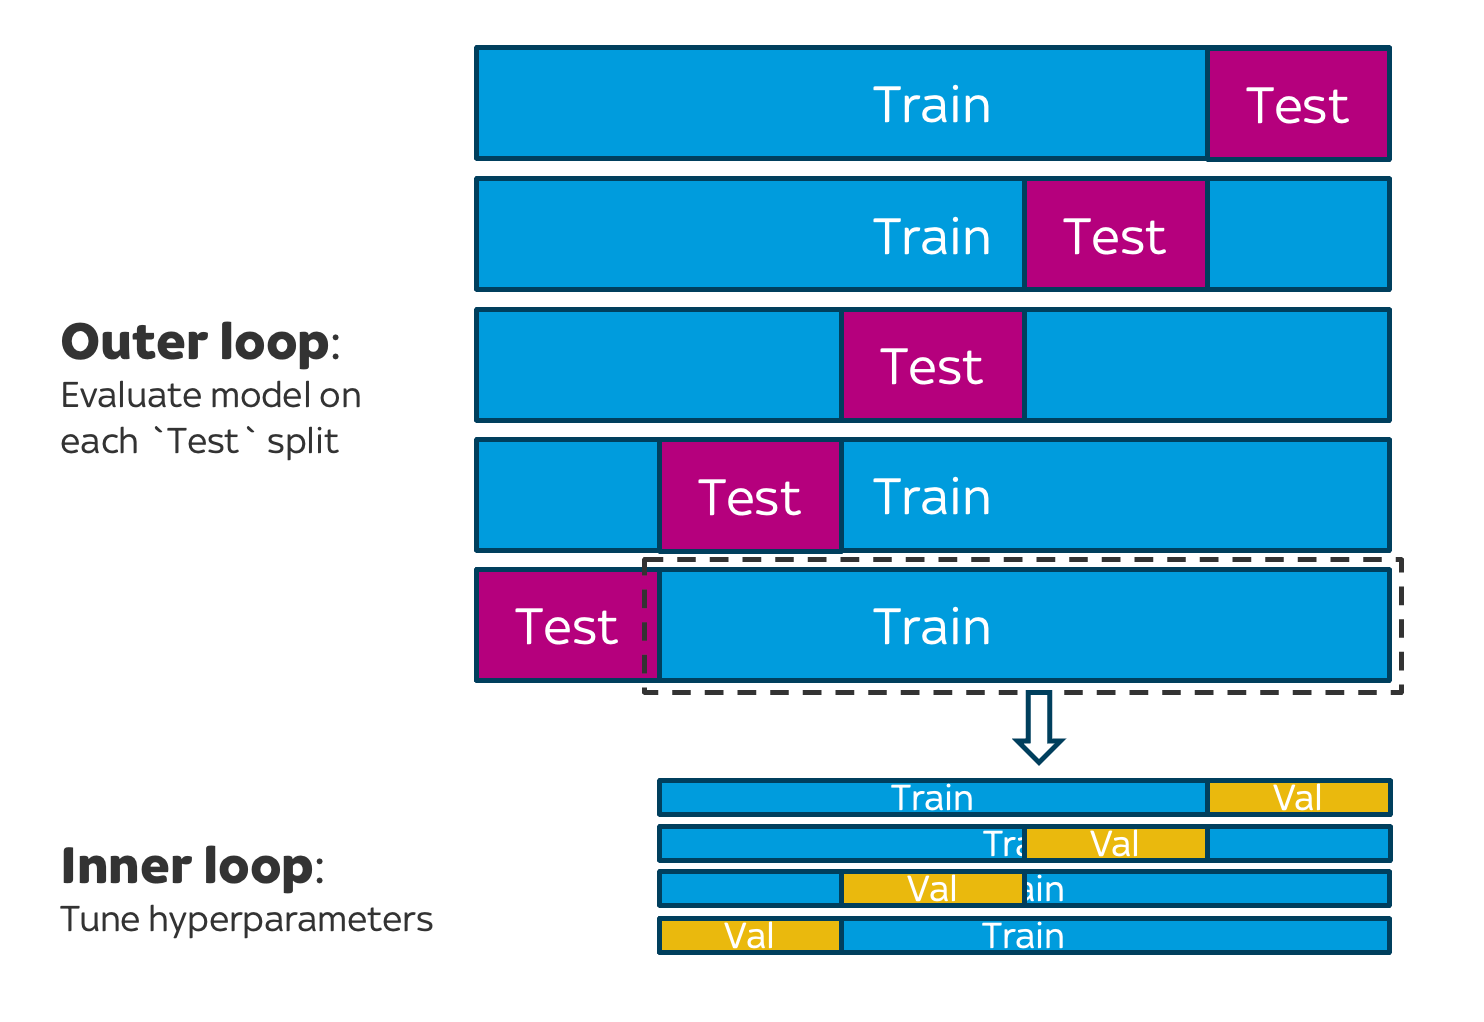
\includegraphics[width = \textwidth]{nested-cv-illustration.png}
        \end{column}
         \begin{column}{0.5\textwidth}
            {\footnotesize
            \begin{itemize}
                \item Test = 2020 (Outer 1)
                \begin{itemize}
                    \item Eval = 2024 (Inner 1.1)
                    \item Eval = 2008 (Inner 1.2)
                    \item ...
                \end{itemize}
        
                \item Test = 2004 (Outer 2)
                \begin{itemize}
                    \item Eval = 2020 (Inner 2.1)
                    \item Eval = 2008 (Inner 2.2)
                    \item ...
                \end{itemize}
            \end{itemize}}
        \end{column}
    \end{columns}

\textbf{Outer:} Grouped Leave One Euro Out (6 Splits)

\textbf{Inner:} Grouped Leave One Euro Out  (5 Splits x 6 Splits = 30 )


\textbf{Image Source:} https://towardsdatascience.com/two-common-pitfalls-to-avoid-when-doing-cross-validation-c68ed79c0e4e/
  

\end{frame}
% ------------------------------------------------------------------
% ------------------------------------------------------------------

\begin{frame}
    \frametitle{Neural Network: Direct Classification}

    \begin{itemize}
        \item Match Result Classification:
        \begin{itemize}
            \item Direct Match Outcomes
            \item Using intermediary Estimated Goals
        \end{itemize}
        \item Classification based on predicted outcome probabilities.
    \end{itemize}

    \vspace{0.4em}

            \centering
            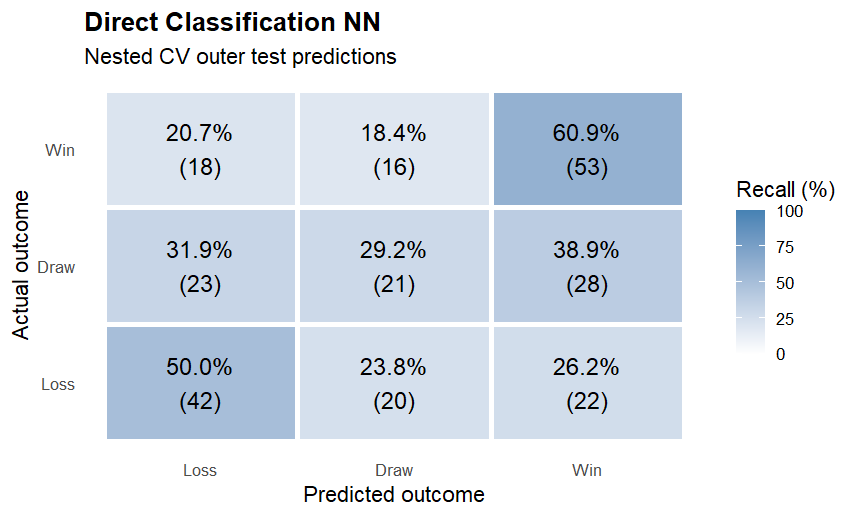
\includegraphics[width=240pt]{directclassification_NN.png}

            \scriptsize
            Direct classification confusion matrix.


    \vspace{0.8em}

    \scriptsize
    Leave-one-tournament-out CV over all 6 tournaments:
    $72 \times 6 = 432$ fits.

\end{frame}

\begin{frame}
    \frametitle{Neural Network: Draw Threshold Tuning}

    \begin{itemize}
        \item Underpredicting draws 
        \item Introducing Recall as a measure of accuracy 
        \item Introducing Draw threshold as a parameter 

    \end{itemize}

    \vspace{0.5em}

            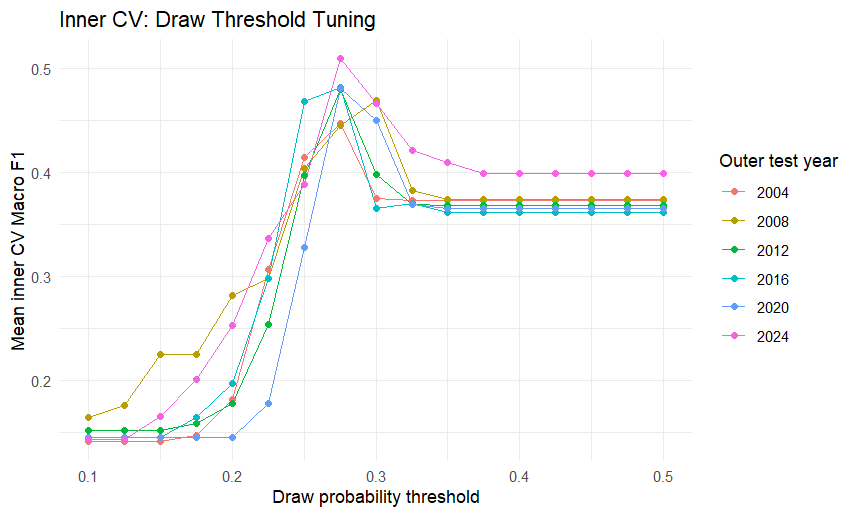
\includegraphics[width=250pt]{Draw Threshold Wider.png}


        


\end{frame}


% ------------------------------------------------------------------
% ------------------------------------------------------------------
\begin{frame}
  \frametitle{Random Forest}

  \begin{columns}[T]

    \begin{column}{0.48\textwidth}
      \textbf{Hyperparameter candidates}

      \vspace{0.4em}
      \footnotesize
      \begin{tabular}{ll}
        \toprule
        \texttt{mtry}              & 1, 2, 3, 4, 5, 6 \\
        \texttt{min.node.size}     & 3, 5, 10, 15 \\
        \texttt{sample.fraction}   & 0.7, 0.85, 1.0 \\
        \bottomrule
      \end{tabular}

      \vspace{0.8em}
      \scriptsize
      Number of trees fixed at 1000.

      \vspace{0.4em}
      Leave-one-tournament-out CV over all 6 tournaments:
      $72 \times 6 = 432$ fits $\rightarrow$ final model.

    \end{column}

    \begin{column}{0.48\textwidth}
      \textbf{Final model}

      \vspace{0.4em}
      \footnotesize
      \begin{tabular}{lr}
        \toprule
        \texttt{mtry}              & 1 \\
        \texttt{min.node.size}     & 15 \\
        \texttt{sample.fraction}   & 0.7 \\
        \texttt{num.trees}         & 1000 \\
        \bottomrule
      \end{tabular}

      \vspace{0.8em}
      \footnotesize
      \begin{tabular}{lr}
        \toprule
        MAE         & 0.836 \\
        RMSE        & 1.045 \\
        Poisson NLL & 1.365 \\
        \bottomrule
      \end{tabular}

      \vspace{0.4em}
      \scriptsize
      Mean six-fold leave-one-tournament-out CV scores
      of the selected combination.

    \end{column}

  \end{columns}

\end{frame}


% ------------------------------------------------------------------
\begin{frame}
  \frametitle{XGBoost}

  \begin{columns}[T]

    \begin{column}{0.48\textwidth}
      \textbf{Hyperparameter candidates}

      \vspace{0.4em}
      \footnotesize
      \begin{tabular}{ll}
        \toprule
        \texttt{max\_depth}         & 1, 2, 3 \\
        \texttt{eta}                & 0.01, 0.05, 0.1 \\
        \texttt{subsample}          & 0.5, 0.8 \\
        \texttt{min\_child\_weight} & 1, 5, 10 \\
        \midrule
        \multicolumn{2}{l}{$3 \times 3 \times 2 \times 3 = 54$ combinations} \\
        \bottomrule
      \end{tabular}

      \vspace{0.8em}
      \scriptsize
      \texttt{nrounds} chosen by early stopping.

      \vspace{0.4em}
      Leave-one-season-out over all 6 seasons:
      $54 \times 6 = 324$ fits $\rightarrow$ final model.
    \end{column}

    \begin{column}{0.48\textwidth}
      \textbf{Final model}

      \vspace{0.4em}
      \footnotesize
      \begin{tabular}{lr}
        \toprule
        \texttt{max\_depth}         & 1 \\
        \texttt{eta}                & 0.1 \\
        \texttt{subsample}          & 0.8 \\
        \texttt{min\_child\_weight} & 5 \\
        \texttt{nrounds}            & 86 \\
        \bottomrule
      \end{tabular}

      \vspace{0.8em}
      \footnotesize
      \begin{tabular}{lr}
        \toprule
        MAE         & 0.828 \\
        RMSE        & 1.035 \\
        Poisson NLL & 1.353 \\
        \bottomrule
      \end{tabular}

      \vspace{0.4em}
      \scriptsize
      Leave-one-season-out CV score of the selected combination.
    \end{column}

  \end{columns}

\end{frame}


% ------------------------------------------------------------------
\begin{frame}
    \frametitle{Poisson Elastic Net 1}

    \small

    \textbf{Hyperparameter Grid} $7 \times 7$ = 49 combinations

    {\footnotesize
    \begin{columns}[c]
        \begin{column}{0.38\textwidth}
            \begin{align*}
                \text{penalty} \in \{&
                1.00e\text{-}10,\;
                4.64e\text{-}09,\;
                2.15e\text{-}07,\\
                &1.00e\text{-}05,\;
                4.60e\text{-}04,\;
                2.15e\text{-}02,\;
                1.00
                \}
            \end{align*}
        \end{column}

        \begin{column}{0.06\textwidth}
            \centering
            $\times$
        \end{column}

        \begin{column}{0.32\textwidth}
            \begin{align*}
                \text{mixture} \in \{&
                0.000,\;0.167,\;0.333,\;0.500,\\
                &0.666,\;0.833,\;1.000
                \}
            \end{align*}
        \end{column}
    \end{columns}
    }

    \textbf{Poisson Regression}
    \vspace{-.2cm}
    \begin{align*}
        \log(\mu(x)) &= \beta_0 + \beta^T x\\
        \ell(\beta|X,Y) &= \sum_{i=1}^N
        \left[
        y_i(\beta_0+\beta^Tx_i)
        - e^{\beta_0+\beta^Tx_i}
        \right]
    \end{align*}

    \vspace{-0.2cm}

    \textbf{Penalized Objective}

    \vspace{-0.1cm}

    \footnotesize
    \[
    \begin{aligned}
    \hat{\beta} = \arg\min_{\beta_0,\beta}
    \quad &-\frac{1}{N}\ell(\beta|X,Y) +\lambda\left[
    \frac{1-\alpha}{2}\sum_{j=1}^p\beta_j^2
    +\alpha\sum_{j=1}^p|\beta_j|
    \right]
    \end{aligned}
    \]

    \vspace{-0.3cm}

    \begin{itemize}
        \item \textbf{Penalty ($\lambda$):} Total amount of regularization.
        \item \textbf{Mixture ($\alpha$):} Proportion of L1 regularization.
        \begin{itemize}
            \item $\alpha=1$: Pure lasso
            \item $\alpha=0$: Ridge regression
        \end{itemize}
    \end{itemize}

    \vfill

    \tiny
    \href{https://glmnet.stanford.edu/articles/glmnet.html\#poisson-regression-family-poisson}{glmnet Poisson regression documentation link}

    \href{https://parsnip.tidymodels.org/reference/poisson_reg.html}{parsnip Poisson regression documentation link}

\end{frame}

\begin{frame}
    \frametitle{Poisson Elastic Net 2}

     \begin{columns}[c]
        \begin{column}{0.2\textwidth}
            \textbf{Best Model:}
                \begin{itemize}
                \item Penalty: .0215
                \item Mixture: 1 
                \end{itemize}
            \textbf{RMSE:} 
                \begin{itemize}
                \item 1.02937 
                \end{itemize}
        \end{column}
        \begin{column}{0.8\textwidth}
            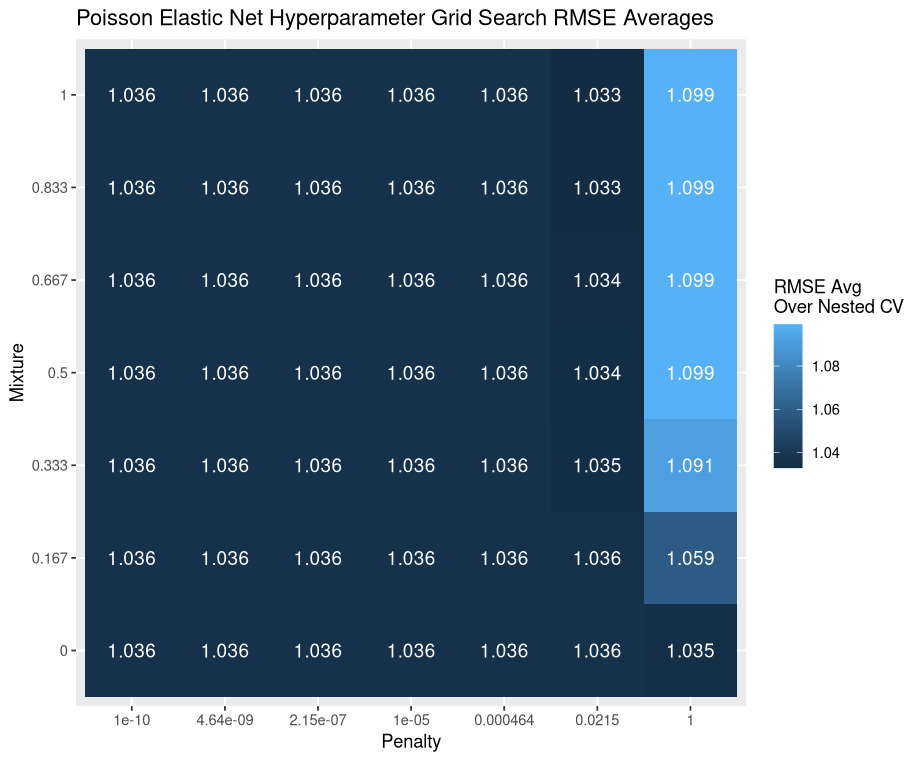
\includegraphics[width = \textwidth]{poisson-grid-search.png}
        \end{column}
    \end{columns}
\end{frame}
 
% ------------------------------------------------------------------
\begin{frame}
  \frametitle{Model Comparison}

  Nested cross-validation: outer loop over the 6 seasons, hyperparameters
  tuned in an inner leave-one-season-out loop. Same folds for every model.


  \vspace{1em}
  \begin{center}
  \begin{tabular}{lcccc}
    \toprule
    Metric & XGBoost & Random Forest & Neural Network & Poisson Reg. \\
    \midrule
    MAE         & 0.831 & 0.8336 & & 0.8236*\\
    RMSE        & 1.038 & 1.0463 & & 1.0294*\\
    Poisson NLL & 1.356 & 1.3622 & & TBD\\
    \bottomrule
  \end{tabular}
  \end{center}

  {\footnotesize
    Note: Poisson Reg. Errors were calculated without taking varying fold sizes into account--to be fixed}
\end{frame}

\end{document}